\documentclass{llncs}

\usepackage[T1]{fontenc}
\usepackage{amssymb, amsmath}
\usepackage{makeidx}
\usepackage{graphicx}
\usepackage{tikz}
\usepackage{standalone}
\usepackage{url}
\usepackage{wrapfig}
\usepackage{array}
\usepackage[hidelinks]{hyperref}
\usepackage{enumitem}

\usepackage{footnote}

\makesavenoteenv{table}

\usetikzlibrary{calc,trees,positioning,arrows,chains,shapes.geometric,%
  decorations.pathreplacing,decorations.pathmorphing,shapes,%
  decorations.text, fit, shapes.geometric, hobby, backgrounds, calc,
  matrix,shapes.symbols,plotmarks,decorations.markings,shadows}

\newcommand{\ignore}[1]{}
\newcommand\todo[1]{\textcolor{blue}{[TODO: #1]}}
\newcommand\TODO[1]{\textcolor{blue}{\small [TODO: #1]}}

\makeatletter
\newcommand\footnoteref[1]{\protected@xdef\@thefnmark{\ref{#1}}\@footnotemark}
\makeatother

%
\begin{document}
%
\mainmatter
%
\title{Automatic Generation of Geographically Accurate Transit Maps}
%
\titlerunning{Automatic Generation of Transit Maps}
%
\author{Hannah Bast\inst{1} \and Patrick Brosi\inst{1} \and
Sabine Storandt\inst{2}}
%
\authorrunning{Hannah Bast et al.} % abbreviated author list (for running head)
%
%%%% list of authors for the TOC (use if author list has to be modified)
\tocauthor{Hannah Bast, Patrick Brosi, Sabine Storandt}
%
\institute{University of Freiburg (Germany)\\
\email{\{bast,brosi\}@informatik.uni-freiburg.de}
\and
JMU W\"urzburg (Germany)\\
\email{storandt@informatik.uni-wuerzburg.de}
}

\maketitle

\begin{abstract}
	We present LOOM, an algorithm for the fully automatic generation of esthetically pleasing and geographically accurate transit maps.
	The input to our algorithm is data about the lines of a given transit network, namely for each line, the sequence of stations it visits and the 
	geographical course the vehicles of this line take.
	%We parse this data from GTFS, the prevailing standard for public transit data.
	%
  %LOOM proceeds in three steps:
	%(1) construct a line graph that captures the topology of the final map;
	%(2) construct an ILP such that an optimal solution yiels a line ordering for each edge which is esthe
	%
	%compute an optimal line ordering for each edge via a suitable constr
	%
	%
	%%ith nodes representing the places where line crossings can occur in the drawing;
	%(2) given the graph, construct an ILP such that an optimal solution to that ILP yields an esthetically pleasing transit map;
	%(3) based on the ILP solution, draw the map.
	%
	We evaluate our algorithms on the GTFS data of six cities around the world.
	The construction process is fast (less than 30 seconds, even for large cities), and the resulting transit maps are esthetically pleasing.
	Indeed, they are surprisingly close to hand-made transit maps and superior to the automatic transit maps provided by Google Maps.
	Previous research work has focused on minimizing the number of line crossings irrespective of the geographical course of the lines and without 
	producing actual maps as an end result.
	% seems like keywords are not common in GD publications
	% \keywords{computational geometry, graph theory, optimization}
\end{abstract}

%
\section{Introduction}\label{SEC:intro}
%
Cities with a subway or tram network usually have an iconic map which illustrates the network and is posted at all stations.
Figure \ref{FIG:transitgraphvvs} provides an excerpt from (our version of) the map of the light rail network of the city of Stuttgart.
%\TODO{We should absolutely have a figure with an example of a real map (on the left) and one of our maps (on the right) already Page 2 of the paper. Stuttgart is probably a good candidat for this, right?}
These maps have to satisfy the following main criteria:\\[-3mm]

\noindent
1. They should accurately depict the topology of the network from the point of view of a public transit user: which lines are available, which stations do they serve in which order, and which transfers are possible.

\smallskip\noindent
2. The map should be neatly arranged and esthetically pleasing (because very many people will look at it every day).

\smallskip\noindent
3. The map should reflect the geographical course of the lines at least to some extent.

\smallskip\noindent
So far, such maps have been designed and drawn by hand.
Concerning 3, they usually take some liberty, either to make the map fit into a certain format or to simplify the layout, or both.
Some maps also have an artistic touch to them.

The goal of this paper is to produce such maps fully automatically, but adhering to 3 rather strictly: within a given tolerance, the lines on the map should be drawn according to their geographical course.


\begin{figure}[t]
  \centering
  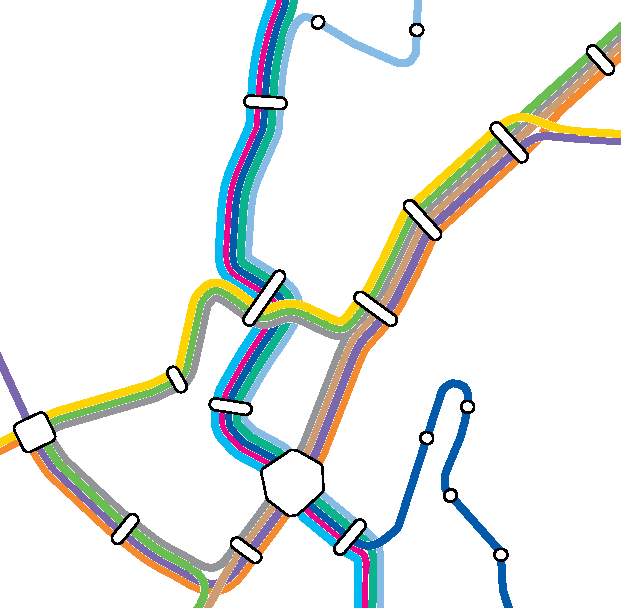
\includegraphics[trim={0cm 0 2.47cm 4.07cm},clip,width=0.44\textwidth]{render_examples/vvs_cropped.pdf}
  \hspace{1.0cm}
	\includestandalone[trim={19pt, 3pt, 0, 0}, clip, width=0.44\textwidth]{render_examples/vvs_transit_graph}
	\caption{Left: An excerpt from our transit map for the light rail network of the city of Stuttgart from 2015 (which happens to look very similar to the actual map of the transit agency). Right: The corresponding excerpt from the line graph which LOOM constructs from the given line data. Each edge corresponds to a segment of the line network, where the same set of lines take the same geographical course. Segment boundaries are often station nodes (large) but can also happen at intermediate nodes (small). The ordering of the lines for each edge (computed in LOOM's central optimization step) determines how the lines are drawn in the final map, and where crossing are necessary.}
		%transit graph of the light rail network in Stuttgart (2015), with embedded lines. Non-station nodes are smaller. Right: transit map rendered from graph.}
  \vspace{0mm}
	\label{FIG:transitgraphvvs}
\end{figure}


\def\Hl{\ell}
\subsection{Overview and Definitions}\label{SEC:intro:definition}

LOOM proceeds in three phases, which we briefly describe in the following along with introducing some notation and terminology that will be used throughout the paper.
 %(1) given the line data, construct the line graph; (2) compute an optimal line ordering for each edge via an ILP; (3) from the line graph and the line ordering, render the map.

\smallskip\noindent
{\bf Input:}
The input to LOOM is a set $S$ of stations and a set $L$ of lines.
Each station has a geographic location.
Each line has a unique ID (in our examples, we use numbers), the sequence of stations it visits, and the geographical course between these stations.
This data is usually provided as part of a GTFS feed of a transit network.\footnote{If the information about the geographical course of the lines is missing, a good approximation is to compute shortest paths on the relevant network. However, this is a problem of separate interest and out of scope for this paper.}

%Let $L$ be a set of transit line labels (e.g. `C', `5', `U 4'). We call an undirected graph $T = (V, E, L)$ with vertices $v = (p_v, \sigma_v)$ and edges $e = (u, v, L(e), \tau_e)$ a transit graph. Each node has a role $\sigma_v \in {0, 1}$. If $\sigma_v = 1$, then we call $v$ a station node, otherwise a non-station node. If $\text{deg}(v) > 2$, we say $v$ is a topology node. $L(e)$ is the set of lines that traverse $e$. Additionally, we define $M = \max_{e \in E} \left|L\left(e\right)\right|$ to be the maximum number of lines per edge.



\smallskip\noindent
{\bf Line graph construction:}
The \emph{line graph} is an undirected labeled graph $G = (V, E, \ell)$, where $V \supseteq S$ (each station is a node, but here may be additional nodes), $E$ is the set of edges, and each $e \in E$ is labeled with a subset $\Hl(e) \subseteq L$ of the lines.
Intuitively, edges correspond to segments of the network, where the same set of lines take the same geographical course (within a certain tolerance, see Section \ref{SEC:graph}), and there is a node wherever a set of lines splits up in different directions.
Figure \ref{FIG:transitgraphvvs} shows the line graph for an excerpt from the network of Stuttgart.
We will see that the complexity of our algorithm depends on $M = \max_{e \in E} |\Hl(e)|$, the maximal number of lines per segment / edge.
The line graph construction is described in Section \ref{SEC:graph}.

\smallskip\noindent
{\bf Line ordering optimization:} 
This phase computes an \emph{ordering} for the line graph, which is simply an ordering of $\Hl(e)$ for each $e \in E$.
This ordering determines where crossing occur, and is hence critical for the appearance of the final map; see again Figure \ref{FIG:transitgraphvvs}.
We formulate this as an Integer Linear Program (ILP).
This phase of LOOM solves a problem that is similar to but distinctly different from the metro-line crossing minimization (MLCM) \cite{bek07} and its variants; this is discussed in Section \ref{SEC:related}.
Section \ref{SEC:ordering} provide the details about this step (in particular, about the ILP).

%Classic MLCM assigns each edge $e$ two orderings $e_{u}$ and $e_{v}$ for $L(e)$, one at each node \cite{nol09}. Line crossings occur somewhere on $e$ if $e_{u} \neq e_{v}$ and crossings inside of nodes are suppressed. We propose an alternative model where only a single ordering is imposed on $L(e)$. This effectively disallows crossings on edges. Instead, we explicitly allow them in nodes (and favor crossings in non-station nodes, see Sect.~\ref{SEC:crossing_placement}). We call this the MLTCM problem, the additional T stands for topology. In our opinion, this model better resembles the way transit maps are drawn manually. In real-world maps, crossings usually occur at nodes where the network topology changes, even if that node is a station. The model also makes for a simple rendering process (Sect.~\ref{SEC:rendering}).
%
%Both problems have the same complexity. MLTCM is reducible to MLCM by transforming every edge $e$ with lines $L(e)$ into a single node $v_e$ with $2\left|L\left(e\right)\right|$ ports. In the next step, all original nodes are replaced by edges that connect those $v_e$ and $n_f$ for which there existed a continued line from $e$ to $f$ via $n$ in the original graph. Similarly, MLCM can be reduced to MLTCM by replacing each edge with a single node and each node with edges between all adjacent original edges with shared lines.
%As a consequence, since MLCM is known to be NP-hard, also MLTCM is NP-hard.

\smallskip\noindent
{\bf Rendering:} 
Given a line graph and an ordering, the final step is to draw the transit map.
Each station node $v$ is drawn as a polygon, where each side of the polygon corresponds to exactly one incident edge of $v$.
We call this side the \emph{node front} of that edge at that station.
The node front for an edge $e$ has $|\Hl(e)|$ so-called \emph{ports}.
Drawing the maps then amounts to connecting the ports (according to the ordering computed in the previous step) and drawing the station polygons.
Note that, just like in previous work, crossing must be explicitly visible and may not be ``hidden'' under stations.
This is crucial such that individual lines can be easily traced through the network.
Section \ref{SEC:rendering} provides more details.

%Optionally, we may assign each $v$ a position $p_v \in \mathbb{R}^2$ and each edge $e$ a polygonal chain $\tau_e = (p_1, ..., p_n), p_i \in \mathbb{R}^2$ which describes the edge's geometrical path. For each $e$, we then require $p_1 = p_u$ and $p_n = p_v$. Each $v$ can be represented by a polygon at which each incident edge $e$ has its own side.  We call this side the node front of $e$ and give it $\left|L\left(e\right)\right|$ ports, one for each line (Fig.~\ref{FIG:crossings}).

%Our goal is to render $T$ as a modern transit map (Fig.~\ref{FIG:transitgraphvvs}). We want to globally optimize the ordering in each $L(e)$ so that single lines can be easily traced through the network. This is usually formulated as the problem of minimizing the number of line crossings in the map and called the Metro Line Crossing Minimization Problem (MLCM).


\subsection{Contributions}\label{SEC:intro:contrib}

We consider the following as our main contributions and ideas:

\vspace{0mm}
\begin{itemize}[parsep=0.5mm,leftmargin=0mm,itemindent=4mm]
\renewcommand\labelitemi{$\bullet$}

\item A new algorithm, called LOOM (Line-ordering-optimized Maps) for the automatic generation of esthetically pleasing and geographically accurate transit maps. The input is basic schedule data as provided in a GFTS feed.

\item This is, as far as we can tell, the first research paper on this problem. Previous research work considers a sub-problem of this task (ignoring the geographical course of the lines). For previous applied work no publications of the details of the underlying algorithm exist. See Section \ref{SEC:related}.

\item Our approach resolves some issues with the MLCM model, in particular, the restricted applicability of some algorithms to planar graphs, and the necessity of artificial grouping of crossings (which happens naturally with our approach).
Also, unlike previous work, we do not only take crossings into account but also separation (that is, lines which are drawn right next to each other in some segment, but have other lines drawn between them in an adjacent segment).
See again Section \ref{SEC:related}.

%\item The main idea underlying LOOM is to construct a \emph{line graph}, where the edges are labeled with lines and the nodes are a superset of the set of stations such that the map can be rendered geographically accurate with line crossings occurring only at nodes (Section \ref{SEC:topo}). An optimal placement of the crossings is then determined via an Integer Linear Program (ILP) constructed from this graph (Section \ref{SEC:ordering}). This information is then used for an esthetically pleasing drawing of the map (Section \ref{SEC:rendering}).
% This approach might also be suited for other graph drawing problems; see Section \ref{SEC:conclusions}.

\item We evaluate LOOM on the transit network of six cities around the world, including New York City. For each city, our algorithm takes below one minute in total. The resulting maps look surprisingly close to hand-made transit maps and superior to the automatic transit maps provided by Google Maps.\footnote{For New York City, the transit maps from Google Maps looks conspicuously better than for other cities. We assume that this particular map has been constructed or at least improved manually.}

\item Our maps are publicly available under \url{loom.cs.uni-freiburg.de} . In particular, the maps there can interactively toggle the display of stations, edges, and node connections. This helps understanding the line graph of LOOM and how the final map is generated from it.

%\item \TODO{mention usefulness, mention bad google maps etc}
%
%\item \TODO{mention that we know of no publication address the MCLM or the drawing of metro maps that uses real-world data}
%
%\item \TODO{mention that we not only want to generate schematic maps, but maps that resemble the real-world vehicle paths as closely as possible} 

\end{itemize}



%\begin{itemize}
	%\item mention usefulness, mention bad google maps etc
	%\item mention that we know of no publication address the MCLM or the drawing of metro maps that uses real-world data
	%\item mention that we not only want to generate schematic maps, but maps that resemble the real-world vehicle paths as closely as possible (e.g. to serve as a map overlay)
	%% see for example Gronemann et al., "Crossing Minimization in Storyline Visualization"
%\end{itemize}

%%
%\subsection{Contribution}\label{SEC:contrib}
%%
%
%We describe an approach for automated drawing of transit maps that can be used with arbitrary schedule data as input. For medium sized urban rail networks, rendering usually only takes a few seconds. A crucial difference of previous approaches to our work is the strong abstraction from the geometry of the transit map. In prior publications, the graph used for optimization is constructed upon the stations which serve as nodes and the transit lines which induce edges between those nodes. But the original embedding of the edges is not taken into account, and crossings are allowed to occur anywhere along the edges (except their endpoints). As we aim for a truthful presentation of vehicle paths in our map, we do not ignore the shape of the lines between stations. Instead, we introduce a new graph model for transit maps where nodes represent topology changes in the embedding and edges represent parallel line segments. This allows us to restrict crossing events to nodes (without hiding them behind station markers!). Our approach resolves some issues with the MLCM model, as e.g. the restricted applicability of some algorithms to planar graphs, and the necessity of artificial grouping of crossings (which happens naturally with our approach).
%
%We describe a line-sweeping approach to extract this graph from a set of (partially overlapping) vehicle trips as they occur in real-world schedule data. To solve the line-crossing problem in our model, we first build a baseline ILP and then develop an improved version of this program. We introduce a line-partner separation constraint and describe an extension to the ILP that optimizes the number of separations. To further simplify the problem, we give some explicit rules to reduce the graph to an optimality-preserving core problem graph.
%
%We also briefly discuss some heuristics for the placement of inevitable crossings and describe how a map can be rendered from our model. Our method is evaluated be running it against several real-world public transit schedules. The maps have been published online\footnote{\url{http://panarea.informatik.uni-freiburg.de/gtfs-lines}}.
%

%
\subsection{Related Work}\label{SEC:related}
%

The problem of minimizing intra-edge crossings in transit maps was introduced in \cite{ben06}, 
with the premises of not hiding crossings under station markers for aesthetic reasons.
A polynomial time algorithm for the special case of optimizing the layout along a single edge was described.
The term metro-line crossing minimization problem (MLCM) was coined in \cite{bek07}.
In that paper, optimal layouts for path and tree networks were investigated but arbitrary graphs were left as an open problem.
In \cite{arg08}, \cite{nol09}, \cite{arg10}, several variants of MLCM were defined and efficient algorithms were presented for some of those, often with a restriction to planar graphs.
In \cite{asq08}, an ILP formulation for MCLM under the periphery condition (see Sec.~\ref{SEC:separation}) was introduced.
The resulting ILP was shown to have a size of $\mathcal{O}(|L|^2 \cdot |E|)$ with $L$ being the set of lines and $E$ the set of edges in the derived graph.
In \cite{fin13b}, it was observed that many (unavoidable) crossings scattered along a single edge are also not visually pleasing, 
and hence crossings were grouped into so-called block crossings.
The problem of minimizing the number of block crossings was shown to be NP-hard on simple graphs just like the original MCLM problem \cite{fin13a}.

All the aforementioned research is oblivious to the geographical course of the lines.
It is also purely theoretical and lacks an experimental evaluation.
There is also some applied work on transit maps, without publications of the details.
One approach that seems to use a model similar to ours was described by Anton Dubreau in a blog post \cite{dub16}.
Google Maps and Here Maps also feature transit maps generated (most likely, automatically) from real data.
However, from an esthetic point of view, these maps are considerably less sophisticated than the maps of Dubreau and our maps.
 %although without a detailed discussion of their method. As far as we are aware there are no papers on MLCM concerned with real data or containing an experimental evaluation.


%
\section{Line Graph Construction}\label{SEC:graph}
%

Public transit data is usually given as a set of vehicle trips. A trip is an ordered list of served stations, optionally given with a geographical path. In recent years, the General Transit Feed Specification (GTFS) has become the dominant format for exchanging schedules\footnote{\url{https://developers.google.com/transit/gtfs/reference/}}. Because each trip is given explicitly, the graph induced by this data has many overlapping edges that may (partially) share the same path. The network topology is usually lost \TODO{what exactly is lost?}.

Let $e_1, e_2$ be two edges in $T$ with their geometrical paths $\tau_{e_1}$ and $\tau_{e_2}$. We define a parametrization $\tau(\lambda): [0,1] \mapsto \mathbb{R}^2$ which maps the progress $\lambda$ to a point $p_d$ on $\tau$. For some distance threshold $\hat{d}$, we say $\left(\left(\lambda_1, \lambda_2\right), \left({\lambda'}_1, {\lambda'}_2\right)\right)$ is a shared segment of $e_1$ and $e_2$ if \[\forall (\lambda, \lambda'), \lambda \in [\lambda_1, {\lambda'}_1], \lambda' \in [\lambda_2, {\lambda'}_2] : \left\|\tau_{e_1}\left(\lambda\right) - \tau_{e_2}\left(\lambda'\right)\right\| \leq \hat{d}.\]

We restore the network topology and transform $T$ into a well-formed transit graph $T'$ by repeatedly combining shared segments between two edges $e_1, e_2$ into a single new edge $e_{12}$ until no more shared segments can be found. If for any of the edges the start of the shared segment $\lambda$ lies not at the beginning of $\tau_e$, we split $e = (u, v)$ at $\lambda$ into two edges $e'$ and $e''$ and introduce a new non-station node $v'$ such that $e' = (u, v')$ and $e'' = (v', v)$ as well as $\tau_{e'}(1) = \tau_{e''}(0) = \tau_{e}(\lambda)$.

To find the shared segments between $\tau$ and $\tau'$, we sweep over $\tau$ in $n$ steps of some $\Delta\lambda$, measuring the distance $d$ between $\tau(i\cdot\Delta\lambda)$ and $\tau'$ at each $i < n$ along the way. If $d \leq \hat{d}$, we start a new segment. If $d > \hat{d}$ and a segment is open, we close it. The algorithm can be made more robust against outliers by allowing $d$ to exceed $\hat{d}$ for a number of $n$ steps. It can be sped up by indexing every linear segment of every path in a geometric index (for example, an R-Tree).

%
\section{Line Ordering Optimization}\label{SEC:ordering}
%

The esthetic appeal of a transit map mostly depends on a clever ordering of the embedded lines.
As described above, we formalize the search for the best ordering as the problem of minimizing the number of line crossings.
Because there are already $\left|L\left(e\right)\right|!$ line permutations for a single edge, the number of ordering configurations even for a small network defies any brute force attack.
For example, the Freiburg tram network (Table~\ref{TBL:datasets}) has roughly $1.13 \cdot 10^{14}$ configurations.
For the Stuttgart network, the number of configurations exceeds the number of atoms in the observable universe by a factor of $10^{27}$.
Finding the optimal configuration is the main challenge in both MLCM and MLTCM.
In this section, we first build a baseline ILP from $T$ to solve MLTCM with $\mathcal{O}(|E| \cdot M^{2})$ variables and $\mathcal{O}(|E| \cdot M^{6})$ constraints. We then define an improved ILP with only $\mathcal{O}(|E|\cdot M^2)$ constraints and describe an extension which solves MLTCM under the line separation constraint.

%
\subsection{Baseline ILP}\label{SEC:baseline}
%
For every edge $e \in E$, we define $\left|L\left(e\right)\right|^{2}$ decision variables $x_{elp} \in \{0,1\}$ where $e$ indicates the edge, $l \in L(e)$ the line, and $p=1, ..., \left|L\left(e\right)\right|$ the position/number of the line in the edge. We want to enforce $x_{elp}=1$ when line $l$ is assigned to edge number $p$ in the edge, and $0$ otherwise. This can be realized as follows:
\begin{equation*}
\forall l \in L(e): \sum_{p=1}^{L(e)} x_{elp}=1.
\end{equation*}
%
To ensure that exactly one line is assigned to each position, we need the following additional constraints:
%
\begin{equation*}
	\forall p \in  \left\{1,...,\left|L\left(e\right)\right|\right\} : \sum_{l \in L(e)} x_{elp} = 1.
\end{equation*}
\subsubsection{Avoiding crossings}\label{SEC:ac}
\begin{figure}[t]
  \centering
	$\vcenter{\hbox{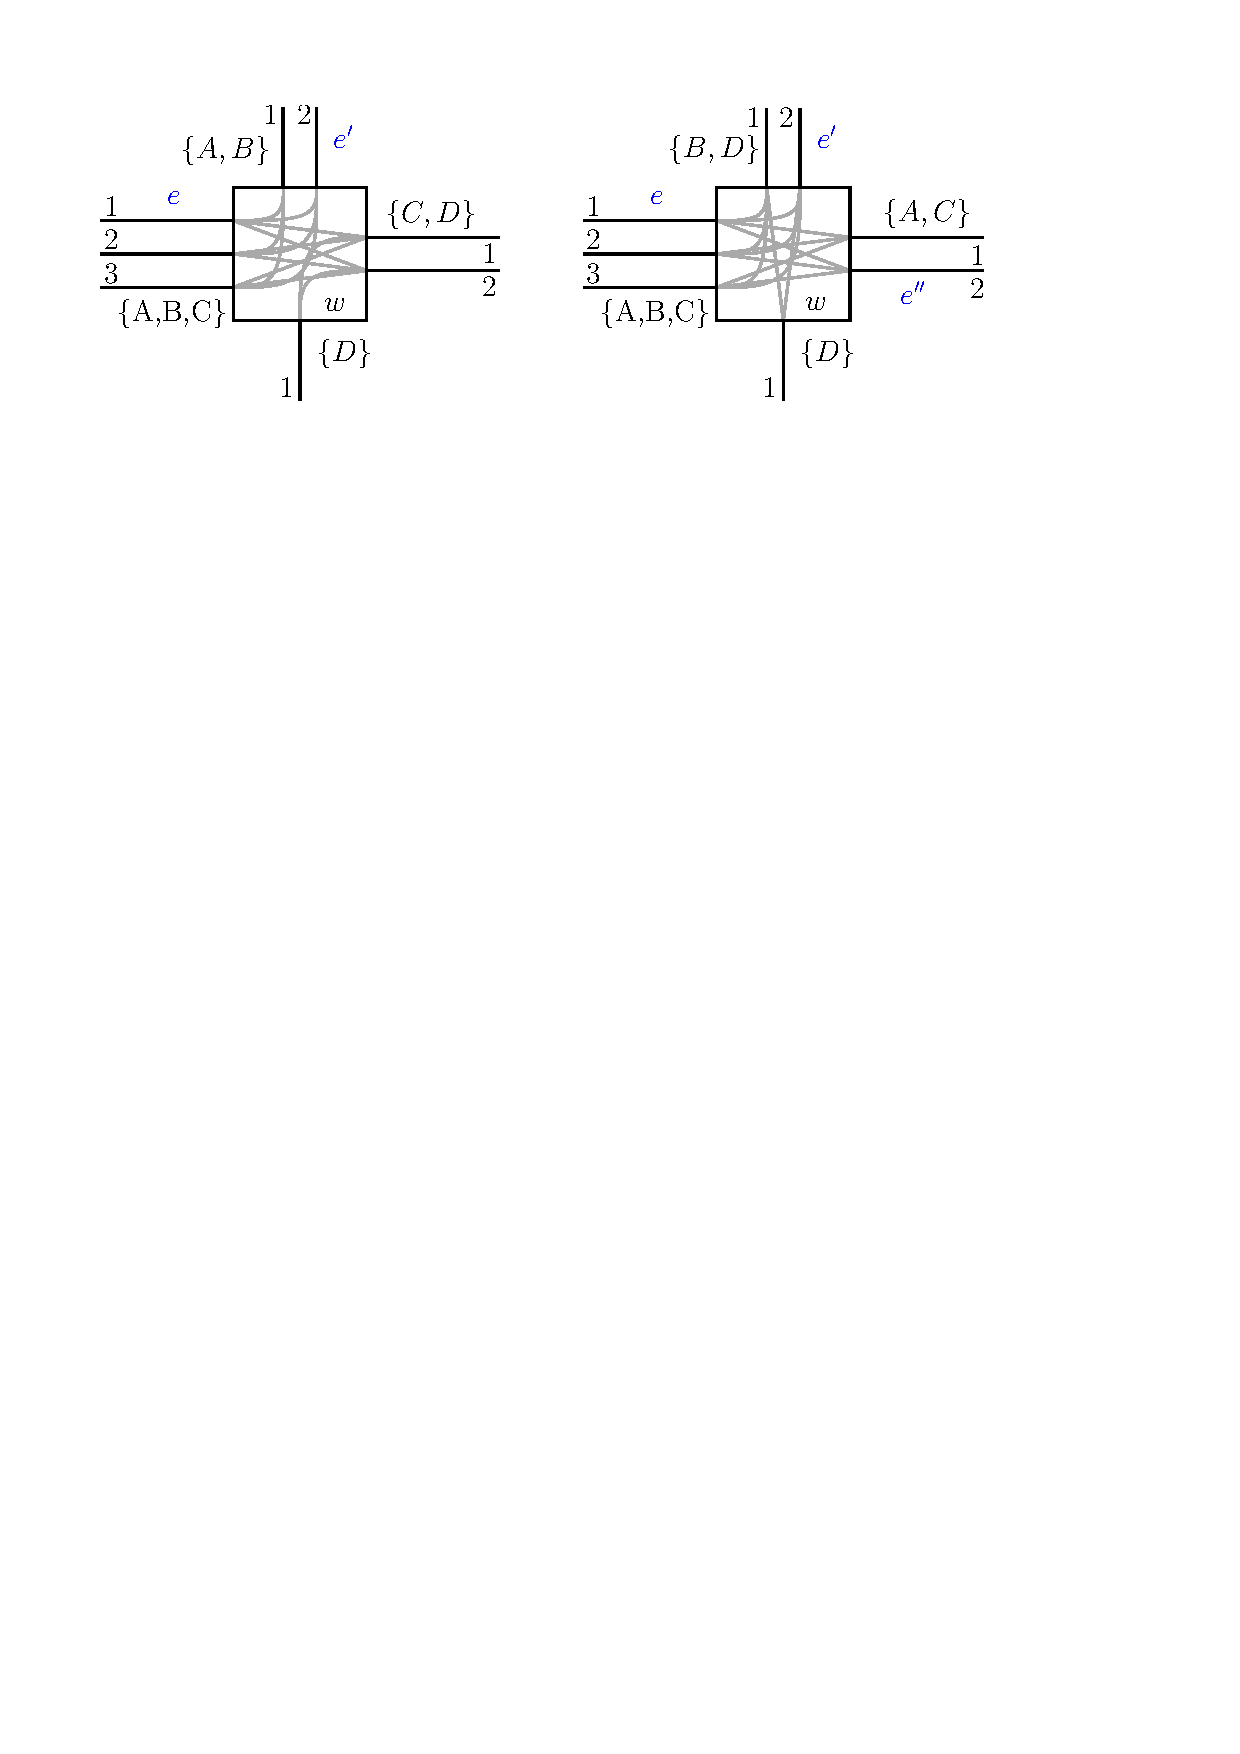
\includegraphics[width=0.8\textwidth]{crossing.pdf}}}$
	\caption{Example instance.}
	\label{FIG:crossings}
\end{figure}
Let $A, B$ be two lines belonging to an edge $e = \{v,w\}$ and both extend over $w$.
We distinguish between two cases: either $A$ and $B$ continue along the same adjacent edge $e'$ (Fig.~\ref{FIG:crossings}, left), or they continue along different edges $e'$ and $e''$ (Fig.~\ref{FIG:crossings}, right).

In the first case, $A$ and $B$ induce a crossing if the position of $A$ is smaller than the position of $B$ in $L(e)$, so $p_e(A) < p_e(B)$, but vice versa in $L(e')$. We introduce the decision variable $x_{ee'AB} \in \{0,1\}$, which should be $1$ in case a crossing is induced and $0$ otherwise. To enforce this, we create one constraint per possible crossing. For example, a crossing would occur if we have $p_e(A)=1$ and $p_e(B)=2$ as well as $p_{e'}(A)=2$ and $p_{e'}(B) =1$. We encode this as follows:
\begin{equation*}
	x_{eA1} + x_{eB2} + x_{e'A2} + x_{e'B1} - x_{ee'AB} \leq 3.
\end{equation*}
In case the crossing occurs, the first four variables are all set to 1. Hence their sum is 4 and the only way to fulfill the $\leq 3$ constraint is to set $x_{ee'AB}$ to $1$. In the example given in Fig.~\ref{FIG:crossings}, six such constraints are necessary to account for all possible crossings of the lines $A$ and $B$ at node $w$.
The objective function of the ILP then minimizes the sum over all variables $x_{ee'AB}$.

In the second case, the actual positions of $A$ and $B$ in $e'$ and $e''$ do not matter, but the order of $e'$ and $e''$ itself \TODO{itself refers to what?}. We introduce a split crossing decision variable $x_{ee'e''AB} \in \{0,1\}$ and constraints of the form
$\quad x_{eAi} + x_{eBj} - x_{ee'e''AB} \leq 1 \quad$
for all orders of $A$ and $B$ at $e$ with $i < j$ because in that case a crossing would occur.
We add $x_{ee'e''AB}$ to the objective function.

\subsubsection{ILP size}
For mapping lines to positions at each edge we need $\leq |E| \cdot M^{2}$ variables and $\leq 2|E| \cdot M$ constraints. To minimize crossings, we have to consider $\leq M^{2}$ pairs of lines per edge, and introduce a decision variable for each such pair. That makes $\leq |E| M^{2}$ additional variables, which all appear in the objective function. Most constraints are introduced when two lines continue over a node in the same direction. In that case, we create $\leq \binom{M}{2}^{2} < M^{4}$ constraints per line pair per edge, so $\leq |E| M^{6}$ in total.
In summary, we have $\mathcal{O}(|E|M^{2})$ variables and $\mathcal{O}(|E|M^{6})$ constraints.

%
\subsection{Improved ILP Formulation}\label{SEC:improved}
%
The $\mathcal{O}(|E|M^{2})$ variables in the baseline ILP seem to be reasonable, as indeed $\Omega(|E|M^{2})$ crossings could occur. But the $\mathcal{O}(|E|M^{6})$ constraints are due to enumerating all possible position inversions explicitly. If we could check the statement \emph{position of A on $e$ is smaller than the position of B} efficiently, the number of constraints could be reduced. To have such an oracle, we first modify the line-position assignment constraints.

\subsubsection{Alternative line-position assignment}
Instead of a decision variable which encodes the exact position of a line, we know use $x_{el\leq p} \in \{0,1\}$ which is $1$ if the position of $l$ in $e$ is $\leq p$ and $0$ otherwise. To enforce a unique position, we use the constraints:
\begin{align}
	\forall l \in L(e)~ \forall p \in \{1, ..., \left|L\left(e\right)\right|-1\}: \quad x_{el\leq p} \leq x_{el\leq p+1}. \label{EQ:up_constr}
\end{align}
This ensures that the sequence can only switch from $0$ to $1$, exactly once. To make sure that at some point a $1$ appears and that each position is occupied by exactly one line, we additionally introduce the following constraints:
\begin{align}
	\forall p \in \{1, ..., \left|L\left(e\right)\right|\}: \sum_{l \in L(e)} x_{el\leq p} = p. \label{EQ:01_constr}
\end{align}
So exactly for one line $x_{e.\leq 1} =1$ is true, for two lines $x_{e.\leq 2} = 1$ (of which one has to fulfill $x_{e.\leq 1} =1$) and so on.

\subsubsection{Crossing Oracle}
We reconsider the example from \ref{SEC:ac}, left. Before, we enumerated all possible positions which induce a crossing for $A, B$ at the transition from $e$ to $e'$. But it would be sufficient to have variables which tell us whether the position of $A$ is smaller than the position of $B$ in $e$, and the same for $e'$, and then compare those variables. For a line pair $(A,B)$ on edge $e$ we call the respective variables $x_{eB<A}, x_{eA<B} \in \{0, 1\}$. %Since we introduce these variables for each line pair in $e$, $x_{eA<B}$ will re-appear as $x_{eB>A}$, so we only need $x_{eA>B}$.
To get the desired value assignments, we add the following constraints:
\begin{gather}
	\sum_{p=1}^{\left|L\left(e\right)\right|} x_{eA\leq p} - \sum_{p} x_{eB\leq p} + x_{eB<A} M \geq 0 \\
	x_{eB<A} + x_{eA<B}=1.
\end{gather}
The equality constraints make sure that not both $x_{eA<B}$ and $x_{eB<A}$ can be $1$. If the position of $A$ is smaller than the position of $B$, then more of the variables corresponding to $A$ are $1$, and hence the sum for $A$ is higher. So if we subtract the sum for $B$ from the sum for $A$ and the result is $\geq 0$, we know the position of $A$ is smaller and $x_{eB<A}$ can be $0$. Otherwise, the difference is negative, and we need to set $x_{eB<A}$ to $1$ to fulfill the inequality. It is then indeed fulfilled for sure as the position gap can never exceed the number of lines per edge.

To decide if there is a crossing, we would again like to have a decision variable $x_{ee'AB} \in \{0,1\}$ which is $1$ in case of a crossing and $0$ otherwise. The constraint
\begin{gather}
	abs(x_{eA<B}-x_{e'A<B}) - x_{ee'AB} \leq 0
\end{gather}
realizes this, as either $x_{eA<B} = x_{e'A<B}$ (both $0$ or both $1$) and then $x_{ee'AB}$ can be $0$, or they are unequal and hence the absolute value of their difference is $1$, enforcing $x_{e'AB}=1$. As absolute value computation can not be part of an ILP we use the following equivalent standard replacement:
\begin{align}
	x_{eA<B} - x_{e'A<B} - x_{ee'AB} &\leq 0 \label{EQ:abs_upper}\\
	-x_{eA<B} + x_{e'A<B} - x_{ee'AB} &\leq 0. \label{EQ:abs_lower}
\end{align}
%If the values are equal, nothing changes in the argumentation. If the values are unequal, either (\ref{EQ:abs_upper}) or (\ref{EQ:abs_lower})  will produce a $1$ as the sum of the first two terms, enforcing $x_{ee'AB}=1$ as desired.

\subsubsection{Complexity of the improved ILP}
For the line-position assignment, we need at most $\leq |E|M^{2}$ variables and constraints just like before.
For counting the  crossings, we need a constant number of new variables and constraints per pair of lines per edge (see above).
Hence the total number of variables and contraints in the improved ILP is $\mathcal{O}(|E|M^{2})$.

\subsection{Placement of Inevitable Crossings}\label{SEC:crossing_placement}
In the ILPs described above, the placement of inevitable crossings largely depends on the solver's strategy and/or the input ordering.

As described above, we want to favor crossings in non-station nodes.
We also found that maps appear more well-arranged if we prefer nodes with larger degree as crossing locations. Since these criteria are invariant to the orderings given to the $L(e)$, we can control them by adding a weighting factor $k_{ee'}$ for each $x_{ee'll'}$ in the objective function.

\subsection{Preventing Line Partner Separation}\label{SEC:separation}

So far, we have only considered the number of crossings.
Another relevant criterion for esthetic appeal is that ``partnering'' lines are drawn next to each other.
Fig.~\ref{FIG:linesplitting} and Fig.~\ref{FIG:linesplitting2} provide two examples.
%
\begin{figure}[t]
\centering
\begin{minipage}{.48\textwidth}
  \centering
	
\includegraphics[trim={2.25 0 2.25 0},clip,angle=270,origin=c,width=.25\textwidth]{render_examples/splitting_example_nonopt.pdf}\hspace{19pt}
	
\includegraphics[trim={2.25 0 2.25 0},clip,angle=270,origin=c,width=.25\textwidth]{render_examples/splitting_example.pdf}
	\caption{Crossings are minimized in the left example (1), but the right example with 2 crossings better indicates line pairings.}
	\label{FIG:linesplitting}
\end{minipage}%
\hfill
\begin{minipage}{.48\textwidth}
  \centering
	
\includegraphics[trim={2.25 0 2.25 0},clip,angle=90,origin=c,width=.25\textwidth]{render_examples/splitting_example2_nonopt.pdf}\hspace{19pt}
	
\includegraphics[trim={2.25 0 2.25 0},clip,angle=90,origin=c,width=.25\textwidth]{render_examples/splitting_example2.pdf}
	\caption{Both orderings have the same number of crossings (2), but in the right example the
crossing is done in one pass.}
	\label{FIG:linesplitting2}
\end{minipage}
\end{figure}
In both cases, the problem could be addressed by punishing the separation of lines. For two adjacent edges $e$ and $e'$ and a line pair $(A, B)$ that continues from $e$ to $e'$, if $A$ and $B$ were placed next to each other in $e$ (were partners in $e$) but not anymore in $e'$, we want to add some penalty to the objective function. For this, we introduce a variable $x_{eA\|B} \in \{0, 1\}$. Let $p_{eA}$ be the position of $A$ in $e$ and $p_{eB}$ the position of $B$ in $e$. We want $x_{eA\|B}$ to be $0$ if $\left|p_{e}(A) - p_{e}(B)\right| = 1$ (if they occur next to each other) and $1$ otherwise. As $x_{eA\|B} = x_{eB\|A}$, we define a set $U(e)$ of unique line pairs in $e$ (that is, $(l, l') \in U(e) \Rightarrow (l', l) \not\in U(e)$). To get the desired assignments, we add the following constraints per line pair $(A, B)$ in $U(e)$:
\begin{align}
	\sum_{p=1}^{\left|L\left(e\right)\right|} x_{eA\leq p} - \sum_{p} x_{eB\leq p} - x_{eA\|B} M &\leq 1 \label{EQ:sep_cstr_1} \\
	\sum_{p=1}^{\left|L\left(e\right)\right|} x_{eB\leq p} - \sum_{p} x_{eA\leq p} - x_{eA\|B} M &\leq 1. \label{EQ:sep_cstr_2}
\end{align}
If $|p_{e}(A) - p_{e}(B)| = 1$, then the difference is $\leq 1$ and $x_{eA\|B}$ can be 0. If $|p_{e}(A) - p_{e}(B)| > 1$, then either (\ref{EQ:sep_cstr_1}) or (\ref{EQ:sep_cstr_2}) enforce $x_{eA\|B} = 1$. To prevent the trivial solution where $x_{A\|B}$ is always 1, we introduce the following additional constraint per edge $e$:
\begin{align*}
	\sum_{(l, l') \in U(e)} x_{el\|l'} \leq \binom{\left|L\left(e\right)\right|}{2} - \left|L\left(e\right)\right| - 1,
\end{align*}
as the number of line pairs in $U(e)$ is $\binom{\left|L\left(e\right)\right|}{2}$ and the number of $(l, l') \in U(e)$ that are next to each other is $\left|L\left(e\right)\right| - 1$.

Like in Sect.~\ref{SEC:improved}, we add a decision variable $x_{ee'A\|B}$ to the objective function that should be $1$ if $A$ and $B$ are split between $e$ and $e'$ and $0$ otherwise:
\begin{align*}
	x_{eA\|B} - x_{e'A\|B} - x_{ee'A\|B} &\leq 0 \\
	-x_{eA\|B} + x_{e'A\|B} - x_{ee'A\|B} &\leq 0.
\end{align*}
%If $\left|L\left(e\right)\right| = |L(e')| = 2$, a line separation penalty is not needed for $A$ and $B$ because they will always be next to each other. If only $\left|L\left(e\right)\right| = 2$, we can add $x_{e'A\|B}$ to the objective function directly (and likewise if only $|L(e')|=2$).

Interestingly, punishing line separations also addresses a special case of the periphery condition introduced in \cite{asq08}. In general, this condition holds if lines ending in some node are always drawn at the left- or rightmost position in each incident edge. For nodes with degree $\leq 2$, the periphery condition is always ensured by the line separation constraint (Fig.~\ref{FIG:periphery1}). For other nodes, however, the periphery condition may not be guaranteed anymore (Fig.~\ref{FIG:periphery2}).

\begin{figure}
\centering
\begin{minipage}{.48\textwidth}
  \centering
	
\includegraphics[trim={0 1.22 0 0},clip,width=.7\textwidth]{render_examples/periphery/periphery_example1.pdf}
	\caption{Periphery condition guaranteed by separation constraint.}
	\label{FIG:periphery1}
\end{minipage}%
\hfill
\begin{minipage}{.48\textwidth}
  \centering
	
\includegraphics[trim={0 1.75 0 0},clip,width=.7\textwidth]{render_examples/periphery/periphery_example2.pdf}
	\caption{Periphery condition not guaranteed by separation constraint.}
	\label{FIG:periphery2}
\end{minipage}
\end{figure}

\subsubsection{Complexity}
We add one additional constraint per edge and a constant number of additional constraints and variables per line pair in each edge to the ILP.
Therefore, the total number of variables and constraints remains $\mathcal{O}(|E|M^2)$.

%
\subsection{Core problem graph}\label{SEC:coreprobgraph}
%

It is possible to further simplify the optimization problem. We observe that the minimum number of crossings or separations in $T$ is exactly the number of crossings or separations that are inevitable and have to occur somewhere.
\begin{lemma}
An inevitable crossing or separation between two lines $J$ and $K$ can only exist if there is a node $v_{jk}$ with one of the following properties:
\begin{enumerate}
\item $v_{jk}$ is adjacent to $e : J \not\in L(e) \land K \in L(e')$ and $e' : J \in L(e') \land K \not\in L(e)$. \label{EQ:liaisonnode}
\item $\left|\left\{e \in adj\left(v_{jk}\right) \mid J \in L\left(e\right) \land K \in L\left(e\right)\right\}\right| > 2$. \label{EQ:tnode}
\end{enumerate}\label{L:inevicrossing}
\end{lemma}
\begin{proof} If no such $v_{jk}$ exists, it holds for all $v \in V$ that $J$ and $K$ either both extend over $v$ on the same (two) edges or do not extend over $v$ at all. In the latter case, no crossing (or separation) can occur and we can thus disregard it, which leaves us only with the former case. But if $J$ and $K$ extend over all nodes on the same two edges, then their relative ordering is irrelevant - we can just combine $J$ and $K$ into a new line $I$ and give them an arbitrary global ordering.
\end{proof}
We call nodes that comply to (\ref{EQ:liaisonnode}) a liaison node and nodes that comply to (\ref{EQ:tnode}) a T-node for $J$ and $K$. Additionally, we call a node in which one or more lines end a terminus node. Because of Lemma~\ref{L:inevicrossing}, we can be sure that for each inevitable crossing, there will be either a liaison node or a T-node where the crossing can occur in. Using this, we can greatly simplify the input graph:
\begin{enumerate}
	\item collapse lines that always occur together into a single new line
	\item remove each edge $e = (u, v)$ where $u$ and $v$ are termini for all $l \in L(e)$.
	\item delete each node $v$ with degree 2 and $L(e) = L(e')$ and combine $e = (u, v)$ and $e'=(v, w)$ into a single new edge $ee' = (u, w)$ with $L(ee') = L(e) = L(e')$.
\end{enumerate}
Because we never delete a liaison nor a T-node, these operations preserve optimality. As we only delete nodes with degree 2, they will also not affect the optimality under the penalty heuristic described in Sect.~\ref{SEC:crossing_placement}, since nodes with higher degree are favored there for crossings/separations.
\begin{figure}
\centering
	\includestandalone[width=5.5cm]{tikz/transitgraph_optim}
	\hspace{0.6cm}
	\includestandalone[width=4.4cm]{tikz/coreoptimgraph}
	\caption{Left: transit graph $T$ with 7 lines, Right: core optimization graph of $T$ with highlighted ordering-relevant connected components with more than 1 node.}
	\label{FIG:coreoptimgraph}
\end{figure}
This core problem graph may be further broken down into ordering-relevant connected components using the rules below (Fig.~\ref{FIG:coreoptimgraph}). The subgraphs can then be optimized separately.
\begin{enumerate}
	\item cut each edge $e = (u, v)$ with $\left|L\left(e\right)\right| = 1$ into two edges $e' = (u, v')$ and $e'' = (v'', v)$. Note that $v'$ and $v''$ are not connected.
	\item replace each edge $e = (u, v)$ where $v$ has a degree $>1$ and is a terminus node for each $l \in L(e)$ with an edge $e' = (u, v')$ where $v'$ is only connected to $e'$.
\end{enumerate}

%
\section{Rendering}\label{SEC:rendering}
%
We split the process of rendering a given transit graph into four basic steps, as illustrated in Fig.~\ref{FIG:renderingproc}.
Each $l \in L(e)$ can be rendered by perpendicular offsetting the edge's polyline by $-w\left|L(e)\right|/2 + w\left(p_{e}(A)-1\right)$, where $w$ is the desired line width and. We make room for the line connections between edges by expanding the node fronts (and thus the node polygon).

After that, the line connections in the node can be rendered independently by connecting all port pairs. In our experiments, we used cubic Bezi\'{e}r curves, but for schematic maps a circular arc or even a straight line might be preferable.

For station rendering, we found that the (buffered) convex hull of the station's node fronts yields reasonable results, although with much potential for improvement. We also experimented with rotating rectangles until the total sum of the deviations between each node front orientation and the orientation of the rectangle was minimized. Both approaches can be seen in Fig.~\ref{FIG:transitgraphvvs}.
\begin{figure}
  \centering
  	\begin{picture}(73, 50)
		\put(0,0){
\includegraphics[width=0.21\textwidth]{render_examples/rendering/render_example1.pdf}}
		\put(0,3){(1)}
	\end{picture}
	\hfill
  	\begin{picture}(73, 50)
		\put(0,0){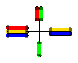
\includegraphics[width=0.21\textwidth]{render_examples/rendering/render_example2.pdf}}
		\put(0,3){(2)}
	\end{picture}
    \hfill
  	\begin{picture}(73, 50)
		\put(0,0){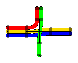
\includegraphics[width=0.21\textwidth]{render_examples/rendering/render_example3.pdf}}
		\put(0,3){(3)}
	\end{picture}
    \hfill
    \begin{picture}(73, 50)
		\put(0,0){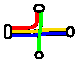
\includegraphics[width=0.21\textwidth]{render_examples/rendering/render_example4.pdf}}
		\put(0,3){(4)}
	\end{picture}
	\caption{The four steps of rendering a given transit graph: (1) render ordered lines as edges, (2) free node area, (3) render inner connections, (4) render station overlays.}
	\label{FIG:renderingproc}
\end{figure}

%
\section{Evaluation}
%

We tested our approach \TODO{give it a name!} on the public transit schedules of four cities: Freiburg, Stuttgart, Chicago, New York.
Table~\ref{TBL:datasets} provides the basic dimensions of each dataset and the time needed to extract the transit graph from the GTFS data.

For each dataset, we consider two versions of the transit graph: the baseline graph and the core optimization graph.
For each graph, we considered three ILP variants: the baseline ILP (B), the improved ILP (I) and the improved ILP under the separation constraint (S).
For each ILP, we evaluated two solvers: the GNU Linear Programming Kit (GLPK) and the COIN-OR CBC solver.

Tests were run on an Intel Core i5-6300U machine with 4 cores \`{a} 2.4 GHz and 12 GB RAM.
The CBC solver was compiled with multithreading support, and used with the default parameters and \texttt{threads=4}.
The GLPK solver was used with the feasibility pump heuristic (\texttt{fp\_heur=ON}), the proximity search heuristic (\texttt{ps\_heur=ON}) and the presolver enabled (\texttt{presolve=ON}).

\def\degv{\text{deg}(v)}
\def\Hms{$\,$ms}
\def\Hs{$\,$s}
\def\Hm{$\,$m}
\def\Hh{$\,$h}
For each node $v$, we added the following penalties to the objective function: $3\cdot \degv$ for each inside-station crossing at $v$, $4\cdot\degv$ for each crossing between line pairs at $v$, and $4\cdot\degv$ for each line separation at $v$ \TODO{reason for the factors 3, 4, 4?}
Note that this counts each crossing or separation event twice: once for once for $(A, B)$, and once for $(B, A)$.
Also note that separations are only considered in ILP variant $(S)$ and disregarded in variants $(B)$ and $(I)$.

\begin{table}
	\caption[]{Dimensions of transit graphs for our six datasets and extraction times from GTFS. $V_{\sigma=1}$ are station nodes, $V_{\sigma=0}$ non-station nodes. $E$ are the graph edges, $L$ the transit lines, and $M$ the maximum number of lines per edge.\label{TBL:datasets}} \vspace{-1ex}
	\centering
	\footnotesize
	\begin{tabular*}{1\textwidth}{@{\extracolsep{\fill}} l r r r r r r r r r r r}
							& & \multicolumn{5}{ c }{\tiny Transit graph} & & \multicolumn{4}{ c }{\tiny Core  optim. graph} \\
							\cline{3-7} \cline{9-12} \\[-2ex] \hline\noalign{\smallskip}
							& $t_{\text{extr}}$ & $|V_{\sigma=1}|$ & $|V_{\sigma=0}|$ & $|E|$ & $|L|$ & $M$ & & $|V|$ & $|E|$ & $|L|$ & $M$ \\
		\noalign{\smallskip}
		\hline
		\noalign{\smallskip}
		Freiburg (Trams)	& 1.54\Hs	& 74	& 6		 & 81	& 5		& 4	&	& 20	& 21	& 5		& 4		\\		
		Dallas (Light Rail) & 9.16\Hs & 108	& 9	 & 118	& 7	& 4	&	& 24	& 24	& 7	& 4		\\
		Chicago	(`L' Train)		& 21.9\Hs	& 143	& 10	 & 154	& 8		& 6	& 	& 23	& 24	& 8		& 6		\\
		Stuttgart (Trams)	& 8.79\Hs	& 192	& 31	 & 235	& 15	& 8	& 	& 51	& 60	& 15	& 8		\\
		Turin (Trams)	  & 28.6\Hs & 339	& 59	 & 435	& 14	& 5	& 	& 89	& 122	& 14	& 5		\\
		New York (Subway)\footnote{with uncollapsed express lines}	& 23.3\Hs & 456	& 61	 & 548	& 26	& 9	&	& 110	& 138	& 23	& 9		\\
		\hline
	\end{tabular*}
\end{table}

\renewcommand*{\thefootnote}{\fnsymbol{footnote}}

\begin{table}
	\caption[]{Sizes of ILPs generated with baseline approach (B), improved approach (I) and added line separation penalty (S), with or without reduction to core graph. Solving times on ``wall-clock''. The numbers of crossings ($\times$) and separations ($||$) as well as the objective value are given after optimization. \label{TBL:evalres}}\vspace{-1ex}
	\centering
	\footnotesize
	\begin{tabular*}{1\textwidth}{@{\extracolsep{\fill}} l l r r r r r r r r r r r r}
							&& \multicolumn{4}{c}{\tiny without core graph reduction} & & \multicolumn{4}{c}{\tiny with core graph reduction} \\
							\cline{3-6} \cline{8-11} \\[-2ex] \hline\noalign{\smallskip}
							&& rows & cols & $t_\text{glpk}$ & $t_\text{CBC}$  & \hspace{4pt} & rows & cols & $t_\text{glpk}$ & $t_\text{CBC}$ & $\times$ & $||$ & obj. \\
		\noalign{\smallskip}
		\hline
		\noalign{\smallskip}
		Freiburg&B    		& 4,034		& 347	 & 198.6\Hs	& 34.2\Hs & & 380	& 124	& 375\Hms	& 717\Hms		& 5		& 1-2\footnoteref{FN:ordering} & 60	\\
		&I 	 				& 641	& 453	 & 484\Hms		& 70\Hms  & & 208	& 160	& \textbf{6\Hms}	& 26\Hms	& 5		& 1-2\footnote[4]{\label{FN:ordering}depended on input ordering and solving strategy} & 60	\\
		&S				& 771	& 514	 & 2.1\Hs		& 2.1\Hs		& & 237	& 173	& \textbf{88\Hms}	& 89\Hms	& 7		& 0	 & 96	\\



		Chicago&B			& 41,242	& 861	 & \textgreater 12\Hh & {\textgreater 12\Hh} & & 8,272 & 266	& \textgreater 12\Hh	& {82\Hm}		& 22 & 4-7\footnoteref{FN:ordering} & 120		\\

		&I					& 1,691	& 1.151	 & 19.6\Hs		& 786\Hms		& & 484	& 352	& \textbf{163}\Hms	& 190\Hms	& 22	& 4-7\footnoteref{FN:ordering}	& 120 \\

		&S				& 2,151	& 1,372	 & (( 25\Hm ))		& 22.3\Hs	& & 595	& 405	& 39.2\Hs	& \textbf{4.5\Hs}	& 27	& 0	& 160	\\



		Stuttgart&B			& 224,396	& 2,455	 & \textgreater 12\Hh& {\textgreater 12\Hh}& & 44,356	& 999	& \textgreater 12\Hh	& \textgreater 12\Hh		& -		& - &	-	\\

		&I 		 			& 5,089	& 3,381	 & (( 12.4\Hm ))		& 4.5\Hs	&	& 1,923	& 1,355 & 10\Hs	& \textbf{400\Hms}	& 65	& 10-15\footnoteref{FN:ordering}	& 276	\\

		&S				& 6,620	& 4,118	 & \textgreater 12\Hh		& 2.3\Hm &	& 2,473	& 1,618	& ??	& \textbf{44.9\Hs}	& 69	& 3	& 426	\\



		New York&B			& 228,596	& 5,181	 & \textgreater 12\Hh& {\textgreater 12 h}& & 95,622		& 2,296	& \textgreater 12\Hh	& \textgreater 12\Hh		& -		& -	& -	\\


		&I 					& 10,575& 7,081	 & (( 6.5\Hh )) 	& 3.1\Hs		& & 4,480	& 3,126	& (( ?? ))	& \textbf{741\Hms}	& 127  	& 9\footnoteref{FN:ordering} & 308	\\


		&S				& 13,518 & 8,482	 & (( ?? ))	& (( 3.7\Hh )) &	& 5,555	& 3,586	& (( ?? ))	& \textbf{76.5\Hs}& 132	& 2	& 382	\\

		\hline
	\end{tabular*}
\end{table}

Table~\ref{TBL:evalres} shows that for (I), the optimal order could be found in under 1 second for each dataset, and for (S) in under 1.5 minutes. For medium-sized networks an optimal solution for (S) was usually found in under $5$ seconds. As expected, core graph reduction made the ILPs smaller. On average, the number of rows decreased by $64\,\%$ and the number of columns by $61\,\%$ for (I). For (S), the average decrease for the number of rows was $60\,\%$ and for the number of columns by $57\,\%$. 
Although the ILPs for (S) were only slightly larger than for (I), optimization on the core graph took $35.4$ times longer on average on COIN.
CBC outperformed glpk for larger datasets, sometimes dramatically. (B) could not be optimized in under $12$ hours for all datasets except Freiburg and Chicago on CBC.
The time needed for graph extraction exceeded the optimization times for most datasets. This is no surprise, as we focused on the line-ordering optimization in this paper. Still, it indicates that further work is necessary here.

%
\section{Conclusions}\label{SEC:conclusions}
%
\TODO{mention thorough aesthetical evaluation via crowd-sourcing?}

\TODO{mention station rendering, which is sub par atm}

\TODO{mention that transit maps are not only useful for transit, but also to visualize for example flowcharts or storylines, layouts of electronic circuits}


\bibliographystyle{plain}
\bibliography{tm}

\end{document}